% !TEX root = main.tex
\chapter{Princípios de Separação Cega de Fontes}
\label{cha:bss}

Antes de iniciar as discussões acerca da tarefa de separação cega de fontes propriamente dita, pode ser interessante realizar uma explicação sobre um cenário básico e generalista. Assim sendo, imagine que haja três diferentes sinais de áudio originais, $s_{1}(t)$, $s_{2}(t)$ e $s_{3}(t)$, que tenham sido emitidos por diferentes fontes de origem, e que, após terem passado por processos de mistura, foram registrados como sinais misturados resultantes por três microfones. Desprezando-se quaisquer outros elementos que possam ser capazes de influenciar diretamente nas misturas, pode-se entender que os sinais resultantes dos processos de mistura são passíveis de serem representados por somas ponderadas dos sinais originais, como mostrado na Equação (\ref{eq:bss_weighted_sum}),

\begin{equation}
\begin{cases}
\begin{aligned}
    x_{1}(t) = a_{11} s_{1}(t) +  a_{12} s_{2}(t) +  a_{13} s_{3}(t) \\
    x_{2}(t) = a_{21} s_{1}(t) +  a_{22} s_{2}(t) +  a_{23} s_{3}(t) \\
    x_{3}(t) = a_{31} s_{1}(t) +  a_{32} s_{2}(t) +  a_{33} s_{3}(t)
    \label{eq:bss_weighted_sum}
\end{aligned}
\end{cases}
\hspace{0.1cm},
\vspace{0.2cm}
\end{equation}

\noindent sendo que $x_{i}$ representa o sinal resultante do processo de mistura, também conhecido como \textit{observação}, e que compõe a matriz de misturas $\mathbf{X}$

\begin{equation}
    \mathbf{\mathbf{X}} =
        \left[
            \begin{array}{c}
                x_{1}(t)    \\
                x_{2}(t)    \\
                \vdots      \\
                x_{m}(t)    
            \end{array}
        \right]
        =
        \left[
            \begin{array}{cccc}
                x_{1}(0) & x_{1}(1) & \cdots & x_{1}(n) \\
                x_{2}(0) & x_{2}(1) & \cdots & x_{2}(n) \\
                \vdots & \vdots & \ddots & \vdots \\
                x_{m}(0) & x_{m}(1) & \cdots & x_{m}(n)
            \end{array} 
        \right];
    \label{eq:bss_mixture_matrix}
\end{equation}

\noindent $a_{ij}$ compreende o peso da ponderação atribuído a cada elemento da mistura, que é um dado inicialmente desconhecido; e $s_{i}$ trata-se do sinal original, que é desconhecido e que é justamente o que se deseja obter ao final de todo o processo e, como de costume, cada sinal é tipicamente compreendido como um processo estocástico estacionário de média zero com valores reais \citep{papoulis1984probability}. Uma versão matricial da Equação (\ref{eq:bss_weighted_sum}) pode ser vista na Equação (\ref{eq:bss_weighted_sum_mat}):

\begin{equation}
    \underbrace{
    \left[\begin{array}{c}
        x_{1}(t) \\
        x_{2}(t) \\
        x_{3}(t)
    \end{array}\right]}_{\mathbf{X}}
    =
    \underbrace{
    \left[\begin{array}{ccc}
        a_{11} & a_{12} & a_{13} \\
        a_{21} & a_{22} & a_{23} \\
        a_{31} & a_{32} & a_{33}
    \end{array}\right]}_{\mathbf{A}}
    \underbrace{
    \left[\begin{array}{c}
        s_{1}(t) \\
        s_{2}(t) \\
        s_{3}(t)
    \end{array}\right]}_{\mathbf{s}}.
    \vspace{0.2cm}
    \label{eq:bss_weighted_sum_mat}
\end{equation}

Isolando-se a matriz de sinais originais, $\mathbf{s}$, será necessário obter a inversa da matriz $\mathbf{A}$, que será tratada como $\mathbf{W}$ neste trabalho, ou seja, $\mathbf{W} = \mathbf{A}^{-1}$, com $\mathbf{W}$ sendo

\begin{equation}
    \mathbf{\mathcal{W}} = \left[ \begin{array}{ccc}
    w_{11} & w_{12} & w_{13} \\
    w_{21} & w_{22} & w_{23} \\
    w_{31} & w_{32} & w_{33} \end{array} \right],
    \vspace{0.2cm}
\end{equation}

\noindent então, pode-se apresentar uma nova formulação que permitirá a obtenção dos sinais originais, desde que algumas condições sejam satisfeitas, que são: a necessidade de o número de observações (sinais resultantes após o processo de mistura) ser superior ao número de fontes (sinais originais); a constatação de uma independência estatística das fontes; a não estacionariedade dos processos de geração dos sinais envolvidos; e o respeito ao limite superior de uma única fonte de distribuição Gaussiana \citep{COMON1994287, romano2010unsupervised}.

Há também a necessidade de a matriz $\mathbf{A}$ ser, de fato, inversível\footnote{Uma forma relativamente prática de verificar tal condição depende apenas do valor do determinante da matriz em questão; caso seja igual a zero, a matriz \underline{não} é inversível.} e, também, a necessidade de a matriz $\mathbf{A}$ ser plenamente conhecida, ou seja, que todos os valores de $a_{ij}$ sejam conhecidos. Em tal situação, pode-se representar o problema da seguinte maneira:

\begin{equation}
    \underbrace{
    \left[\begin{array}{c}
        y_{1}(t) \\
        y_{2}(t) \\
        y_{3}(t)
    \end{array}\right]}_{\mathbf{y}}
    =
    \underbrace{
    \left[\begin{array}{ccc}
        w_{11} & w_{12} & w_{13} \\
        w_{21} & w_{22} & w_{23} \\
        w_{31} & w_{32} & w_{33}
    \end{array}\right]}_{\mathbf{W}}
    \underbrace{
    \left[\begin{array}{c}
        x_{1}(t) \\
        x_{2}(t) \\
        x_{3}(t)
    \end{array}\right]}_{\mathbf{X}},
    \vspace{0.2cm}
    \label{eq:bss_inv_weighted_sum_mat}
\end{equation}

\noindent ou ainda, novamente na forma de um sistema de equações,

\begin{equation}
\begin{cases}
\begin{aligned}
    y_{1}(t) = w_{11} x_{1}(t) +  w_{12} x_{2}(t) +  w_{13} x_{3}(t) \\
    y_{2}(t) = w_{21} x_{1}(t) +  w_{22} x_{2}(t) +  w_{23} x_{3}(t) \\
    y_{3}(t) = w_{31} x_{1}(t) +  w_{32} x_{2}(t) +  w_{33} x_{3}(t)
    \label{eq:bss_inv_weighted_sum}
\end{aligned}
\end{cases}
\hspace{0.1cm}.
\vspace{0.2cm}
\end{equation}

Mas esta é apenas uma visão teórica de uma parte--digamos--mais controlada do problema. O que se tem na prática, efetivamente, é que a tarefa de se obter cada componente em questão pode ser algo impraticável ou, no mínimo, inviável. Assim, antes de partir para a tarefa de identificação dos componentes em si, deve-se realizar um pré-processamento, a ser melhor explicado na Seção \ref{sec:bss_preproc}.



\section{Características dos Modelos}
\label{sec:bss_characteristics}

O problema de separação de sinais não é algo simples de ser resolvido; para compreendê-lo melhor, pode ser muito convidativa a utilização de formas esquemáticas ilustrativas que abordem o problema de um modo mais genérico. Contudo, a utilização de formas generalistas em demasia pode transmitir a errônea impressão de que as técnicas gerais podem ser aplicadas em múltiplos cenários consideravelmente distintos com grau de eficácia equiparável, o que não reflete a realidade. Para se atingir maiores níveis de eficácia e de eficiência, pode ser muito vantajoso compreender especificamente o cenário em que se realizará a separação de fontes e, a partir de modelos que considerem as características inerentes a tal cenário, seja feita a separação. Características relacionadas à linearidade e à memória serão melhor tratadas a seguir.


%   ----- Linearidade -----
\subsection{Linearidade}
\label{subsec:bss_linearity}

De acordo com o Princípio da Superposição, sistemas lineares compostos pela soma de múltiplos estímulos terão como respostas a soma das respostas individuais para cada entrada individual no sistema, assim como a proporção escalar da entrada resultará em igual proporção escalar da saída. Em outras palavras, a soma das entradas em um determinado sistema linear resultará na soma das saídas desse mesmo sistema, respeitando-se as suas respectivas proporções. Vale lembrar que o Princípio da Superposição pode ser matematicamente descrito a partir de duas propriedades conhecidas como Aditividade e Homogeneidade:\\

\begin{definition}[Princípio da Superposição]
    Sejam $\bm{F}(\cdot)$ uma função linear, $\bm{x}$ uma variável de entrada e $\alpha$ um escalar. Assim, a partir das propriedades de Aditividade e Homogeneidade

    \begin{equation*}
        \begin{aligned}
            & \bm{F}(\bm{x}_{1} + \bm{x}_{2}) = \bm{F}(\bm{x}_{1}) + \bm{F}(\bm{x}_{2}) \hspace{0.5cm}& \text{\textbf{Aditividade}} \\
            & \bm{F}(\alpha \bm{x}) = \alpha \bm{F}(\bm{x}) & \hspace{0.5cm} \text{\textbf{Homogeneidade}}
        \end{aligned}
        \vspace{0.2cm}
    \end{equation*}

    \noindent pode-se chegar ao \textbf{Princípio da Superposição}:

    \begin{equation}
        \begin{aligned}
            \bm{F}(\alpha_{1} \bm{x}_{1} + \alpha_{2} \bm{x}_{2}) & = \bm{F}(\alpha_{1} \bm{x}_{1}) + \bm{F}(\alpha_{2} \bm{x}_{2})\\
             & = \alpha_{1} \bm{F}(\bm{x}_{1}) + \alpha_{2} \bm{F}(\bm{x}_{2})
        \end{aligned}
        \hspace{0.1cm}
        \vspace{0.2cm}
    \end{equation}

\end{definition}

Assim sendo, a partir da definição do princípio da superposição, é possível considerar uma analogia para sinais misturados por um processo de mistura como um sistema linear, representado aqui por $\bm{F}(\cdot)$. Considerando, então, os sinais $\bm{s}_{1}[n]$ e $\bm{s}_{2}[n]$ e os escalares $\alpha_{1}$ e $\alpha_{2}$, o modelo linear pode ser representado por

\begin{equation}
    \bm{F}(\alpha_{1} \bm{s}_{1}[n] + \alpha_{2} \bm{s}_{2}[n]) = \alpha_{1} \bm{F}(\bm{s}_{1}[n]) + \alpha_{2} \bm{F}(\bm{s}_{2}[n])
    \hspace{0.1cm}.
    \vspace{0.2cm}
    \label{eq:bss_superpos}
\end{equation}

\noindent Todos os casos que não possam ser corretamente representados por formas análogas advindas de uma generalização feita a partir da Equação (\ref{eq:bss_superpos}) são chamados \textit{não-lineares}. Os casos não-lineares comumente são mais complexos e, assim, demandam o uso de técnicas mais avançadas, além de nem sempre permitirem que resultados com níveis satisfatórios de qualidade sejam alcançáveis por meio das técnicas que geralmente costumam ser exploradas para tais fins. Algumas das técnicas exploradas nesses casos são: ICA Não-Linear, Minimização de Informação Mútua e Gassianização.



%   ----- Memória -----
\subsection{Memória}
\label{subsec:bss_memory}

Uma forma bastante usual de se analisar a questão da memória é separando-a em sistemas sem memória e sistemas com memória, sendo que neste contexto é comum referir-se aos sistemas com memória como sendo sistemas convolutivos, dado que tais sistemas são dependentes de memória, além de serem tipicamente lineares na maior parte dos casos. Sistemas com memória tendem a depender de tratativas importantes para que seja possível realizar implementações dependentes de processamento em tempo real, devido ao fato de serem mais suscetíveis a problemas provocados por atrasos, sobretudo quando os atrasos sofrem variações em um largo intervalo.\\

\begin{definition}[Convolução]
    Sejam $s_{1}[n]$ e $s_{2}[n]$ dois sinais de tempo discreto; a convolução entre eles é definida por:

    \begin{equation}
    \begin{aligned}
        y[n]    & = s_{1}[n] \ast s_{2}[n] \\
                & = \sum_{i=-\infty}^{+\infty} s_{1}[i]\cdot s_{2}[n - i]
    \end{aligned}
    \vspace{0.2cm}.
    \end{equation}

    \noindent Sendo que a convolução possui as propriedades de Associatividade, Comutatividade e Distributividade, apresentadas a seguir:

    \begin{equation*}
    \begin{aligned}
        (s_{1}[n] \ast s_{2}[n]) \ast s_{3}[n] & =  s_{1}[n] \ast (s_{2}[n] \ast s_{3}[n]) & \hspace{0.5cm}\text{\textbf{Associatividade}} \\
        s_{1}[n] \ast s_{2}[n] & = s_{2}[n] \ast s_{1}[n] & \hspace{0.5cm}\text{\textbf{Comutatividade}} \\
        s_{1}[n] \ast (s_{2}[n] + s_{3}[n]) & = s_{1}[n] \ast s_{2}[n] + s_{1}[n] \ast s_{3}[n] & \hspace{0.5cm}\text{\textbf{Distributividade}}
    \end{aligned}
    \vspace{0.2cm}
    \end{equation*}

\end{definition}





%   ----------------------------------
%   ----- Problemas Relacionados -----
%   ----------------------------------
\section{Problemas Relacionados}
\label{sec:bss_correlated_problems}

Além dos pontos até então mencionados ao longo desta seção, existem problemas relacionados ao de BSS e que, por vezes, podem inclusive ser vistos como uma espécie de extensão ou versão decomposta deste primeiro problema central, tais como o de Extração Cega de Fontes, o de Desconvolução e o de \textit{Denoising}; todos eles serão explicadaos a seguir, fazendo-se, contudo, a ressalva a respeito do fato de que um aprofundamento minucioso e um rigoroso detalhamento matemático não fazem parte dos objetivos deste trabalho; assim, caso haja interesse em compreender a fundo as questões mencionadas, sugere-se uma visita aos materiais citados e referenciados.



%   ----- BSE -----
\subsection{Extração Cega de Fontes}
\label{subsec:bss_bse}

Um dos vários problemas relacionados ao de BSS é conhecido como Extração Cega de Fontes (\textbf{BSE}, do inglês \textit{Blind Source Extraction}) \citep{5967775}, sendo justamente um dos mais próximos ao que efetivamente é o próprio problema de BSS, afinal, enquanto o BSS deseja obter a versão separada de todos os sinais de interesse, o BSE almeja fazer algo similar, mas apenas para um sinal, tal como representa o modelo a seguir: \\

\nomenclature{BSE}{\textit{Blind Source Extraction}}

\begin{definition}[Extração Cega de Fontes]

    Sejam $\bm{X}$ uma matriz de misturas observadas e $\bm{w}$ o vetor de extração. O processo de obtenção do sinal $\bm{y}_{i}$ por meio de BSE é definido por

    \begin{equation}
        \bm{y}_{i} = \bm{w}^{T} \bm{X}
        \label{eq:bss_bse}
        \hspace{0.1cm},
        \vspace{0.2cm}
    \end{equation}

    \noindent em que $\bm{y}_{i}$ corresponde ao sinal original da $i$-ésima fonte.

\end{definition}

É importante constatar o fato de que é possível atingir os mesmos objetivos do BSS a partir do uso iterativo de métodos de BSE, que pode utilizar-se de um método chamado Deflação \citep{DELFOSSE199559}. A deflação se trata de um processo que efetua a remoção das contribuições advindas do sinal removido pelo processo de extração, ou seja, ao final de cada iteração concluída do processo de BSE, deve ser realizado o processo de deflação. Desta forma, as misturas restantes não continuarão sob os efeitos oriundos da participação do sinal extraído, fazendo com que possa ser seguido o procedimento reiteradas vezes até que todos os sinais sejam sucessivamente extraídos.



%   ----- Desconvolução -----
\subsection{Desconvolução}
\label{subsec:bss_deconvolution}

O problema de desconvolução, que pode ser compreendido como o de separar sinais convoluídos entre si, ou seja, que passaram pelo processo de convolução, também pode ser visto como um problema de mistura subparametrizada. Aqui vale lembrar que, devido a propriedades da convolução, a ordem com que as convoluções ocorrem é irrelevante para os resultados finais de todo o processo convolutivo. Em casos de trabalhos relacionados a áudio, uma aplicação bastante interessante que é almejada pela desconvolução é o cancelamento de ecos desconhecidos, assim como reverberações indesejadas em sinais de fala; para trabalhos com imagens, um exemplo típico é o de imagens borradas \citep{Bell:1995:IAB:211676.211677}.

Existem duas interpretações comumente adotadas para o termo Desconvolução Cega: a de um cenário em que se conhece apenas um dos sinais envolvidos; e a de um cenário em que absolutamente nenhum dos sinais envolvidos é conhecido, o que faz, portanto, com que a única informação exposta seja a da própria convolução em si. Assim sendo, dada uma mistura observada $y[n]$, presume-se que ela é o resultado de um processo de convolução entre dois sinais $s_{1}[n]$ e $s_{2}[n]$, ou seja, é possível representar o problema da seguinte forma:

\begin{equation}
    y[n] = s_{1}[n] \ast s_{2}[n]
    \label{eq:bss_deconvolution}
    \hspace{0.1cm}.
    \vspace{0.2cm}
\end{equation}

O que se almeja aqui é efetuar essa decomposição, ou seja, obter os sinais $s_{1}[n]$ e $s_{2}[n]$ que, ao serem convoluídos, resultam no sinal $y[n]$. Através das técnicas clássicas de deconvolução não é possível atingir tal objetivo sem que sejam feitas suposições iniciais, mas não basta assumir qualquer realidade para que o algoritmo obtenha êxito em sua aplicação. Os trabalhos \citep{661479, 7077344} ilustram bem dois exemplos de aplicações em áreas de multimídia; mais especificamente, em áudio.


Apesar de ter notoriamente focado em aplicações de processamento de imagens, o trabalho \citep{levin2009understanding} é bastante importante e útil a todos aqueles que desejarem compreender algoritmos de BSE de forma mais aprofundada; ao longo do artigo podem ser vistas análises teóricas e experimentais, incluindo um estudo a respeito do motivo da falha por parte da abordagem que tenta utilizar a estimação de Máximo a Posteriori (\textbf{MAP}, do inglês \textit{Maximum a Posteriori}).






%   ----- Denoising -----
\subsection{Denoising}
\label{subsec:bss_denoising}

O termo \textit{Denoising} remete a tratamento de ruídos, independentemente de quais sejam, de como afetam o objeto de interesse do projeto e de quais devem ser, especificamente, as técnicas a serem utilizadas para realizar tal tarefa, embora saiba-se que uma tratativa estatística será necessária devido à natureza dos ruídos \citep{watkinson2001art}. Supressão de ruídos, tratamento de ruídos, redução de ruídos, atenuação de ruídos, cancelamento de ruídos e remoção de ruídos são apenas alguns dos nomes atribuídos a todo um grande conjunto de técnicas cujos objetivos finais acabam sendo, de alguma maneira, o de diminuir os efeitos nocivos provocados por essas perturbações chamadas neste contexto de \textit{ruídos}.

O trabalho \citep{1163209} traz um algoritmo que efetua um tratamento de ruídos em sinais de voz; mais especificamente, o método suprime os efeitos de ruídos estacionários da fala humana tomando como base os trechos do sinal em que não há fala para se obter o \textit{bias} do ruído espectral envolvido. Mas nem sempre o cenário será o mesmo; diversas características sobre o ambiente e sobre o sistema podem sofrer alterações ao longo do tempo. Assim, pode não ser vantajoso apoiar-se exclusivamente em um modelo pré-definido, fixo e inalterável de solução. Uma proposta mais flexível, que permita adaptações conforme a necessidade, pode ser bem mais convidativa e conveniente; modelo amplamente compreendidos como adaptativos \citep{1451965, 382009}.

Tal como observado em \citep{7805139, 6334422, 1643650, SPRIET20042367}, uma das técnicas clássicas mais exploradas para se tratar ruídos em sinais de áudio é o Filtro de Wiener\footnote{O trabalho havia sido desenvolvido no \textit{Radiation Laboratory}, MIT, alguns anos antes, aproximadamente entre 1940 e 1942, mas foi classificado como secreto na época e, portanto, mantido sob o mais absoluto sigilo, dadas as circunstâncias da época, dado que os propósitos era de estimar a posição dos bombardeiros alemães a partir de reflexos de radares.} \citep{6284754}, que tipicamente explora o Erro Quadrático Médio (\textbf{MSE}, do inglês \textit{Mean Square Error}) como a função custo do problema, almejando-se, portanto, minizá-la para que se possa atingir o mais baixo nível de ruído possível.

\nomenclature{MSE}{\textit{Mean Square Error}}

Mas, apesar de sua enorme contribuição para a área, o filtro de Wiener não podia ser utilizado em qualquer cenário; possuía algumas limitações, como a de depender de processos que fossem estacionários em sentido amplo. Então, vários anos depois, partindo de uma generalização do filtro de Wiener, foi desenvolvido o Filtro de Kalman \citep{kalman1960new}, que pode ser aplicado a processos não estacionários. Tal forma de filtragem obteve ampla adesão nesta área e vários trabalhos foram feitos explorando suas características bastante convenientes, como \citep{701367, 1169756, 91144}.

Além das técnicas mencionadas, há todo um enorme conjunto de outras abordagens, tais como o uso da Transformada Wavelet Discreta (\textbf{DWT}, do inglês \textit{Discrete Wavelet Transform}), geralmente mais explorada em aplicações de imagem e vídeo \citep{119727, doi:10.1175/1520-0477, 336245}; e o da Transformada de Fourier de Tempo Curto (\textbf{STFT}, do inglês \textit{Short-Time Fourier Transform}), bastante utilizadas para áudio \citep{622558, 1164910, 4156182, 1164162, 466662}.

\nomenclature{DWT}{\textit{Discrete Wavelet Transform}}
\nomenclature{STFT}{\textit{Short-Time Fourier Transform}}




%   ---------------
%   ----- ICA -----
%   ---------------
\section{Análise de Componentes Independentes}
\label{sec:bss_ica}

O método de Análise de Componentes Independentes (\textbf{ICA}, do inglês \textit{Independent Component Analysis}) é um dos mais importantes e consagrados métodos de separação de sinais já desenvolvidos até então. É, provavelmente, o método mais amplamente utilizado para as mais diversas aplicações dependentes de um processo de separação de fontes, sobretudo para BSS. O método de ICA pode ser interpretado como uma extensão agregadora do PCA \citep{COMON1994287}, explorando independência estatística em vez de apenas considerar correlação e covariância.

\nomenclature{ICA}{\textit{Independent Component Analysis}}

Apenas como uma questão de curiosidade, é interessante lembrar que uma das conferências internacionais de maior importância na área de separação de sinais trazia os termos ``Independent Component Analysis'' em seu título, certamente que por motivos mais do que justos na época, o que se manteve até o ano de 2009; a partir de então, em vez de disso, por uma questão de generalidade e abrangência, dadas as evoluções na área, compreendeu-se que seria mais conveniente classificar o ICA como um dos possíveis métodos de algo ainda maior, chamado de Análise de Variáveis Latentes\footnote{De modo praticamente oposto às variáveis observáveis, as variáveis latentes são as que não podem ser diretamente aferidas, lidas ou constatadas; em vez disso, são variáveis que dependem de algum tipo de transformação, adaptação ou inferência para que, só então, possam ser obtidas e, enfim, exploradas.} (\textbf{LVA}, do inglês \textit{Latent Variable Analysis}), então o termo que assumiu tal lugar no nome desta importante conferência internacional foi justamente ``Latent Variable Analysis''.

\nomenclature{LVA}{\textit{Latent Variable Analysis}}

Além do ICA, outros métodos que também se encaixam na categoria de LVA são: o Modelo Oculto de Markov (\textbf{HMM}, \textit{Hidden Markov Model}) \citep{18626}, a PCA, a Análise Fatorial (\textbf{FA} e a \textit{Factorial Analysis})\footnote{Análise Fatorial, na verdade, trata-se de um conjunto de técnicas, não de uma única técnica \textit{Stricto sensu}. Isso faz com que não haja um único trabalho específico que possa ser utilizado como a referência; o que há, porém, é uma vasta gama de trabalhos sobre as técnicas propriamente ditas, podendo ser sobre as técnicas em si ou aplicações --comumente, em pesquisas de Psicologia-- que as explorem.} \citep{vincent1953orgin, c63851e778034799a99dcc4d187768d0, doi:10.1177/001316446002000116}.

\nomenclature{HMM}{\textit{Hidden Markov Model}}
\nomenclature{FA}{\textit{Factorial Analysis}}

Partindo agora para a definição do que vem a ser efetivamente o método de ICA, pode-se dizer que, segundo \citep{hyvarinen2004independent}, possuindo-se diretamente apenas os sinais resultantes (misturados), $x_{i}(t)$, o ICA se trata da estimação de dois específicos elementos, que são: a matriz ponderadora $\mathbf{A}$, que é responsável pelos pesos das combinações lineares que neste contexto são convenientemente compreendidas como misturas; e os sinais originais independentes, $s_{i}(t)$, assim como havia sido mostrado no início deste capítulo, também poderiam ser compreendidas na forma de um sistema de equações lineares, tal como

\begin{equation}
\begin{cases}
\begin{aligned}
    s_{1}(t) & = & w_{11} x_{1}(t) +  w_{12} x_{2}(t) + \cdots + w_{1n} x_{3}(t) \\
    s_{2}(t) & = & w_{21} x_{1}(t) +  w_{22} x_{2}(t) + \cdots + w_{2n} x_{3}(t) \\
     & \hspace{0.08cm} \vdots & \\
    s_{n}(t) & = & w_{n1} x_{1}(t) +  w_{n2} x_{2}(t) + \cdots + w_{nn} x_{3}(t)
    \label{eq:bss_ica}
\end{aligned}
\end{cases}
\vspace{0.2cm}
\end{equation}

\noindent porém, apesar de em alguns cenários a visualização do problema na forma de um sistema de equações, tal como pode ser observado em (\ref{eq:bss_ica}), ser mais humanamente conveniente --- talvez por uma questão de hábito ---, as implementações computacionais são dependentes de uma linguagem que esteja de acordo com representações matriciais

Ainda em \citep{hyvarinen2004independent} é sugerido um método alternativo para implementar o ICA, que é encontrando-se uma transformação linear dada por uma matriz $\mathbf{W}$, a mesma da Equação (\ref{eq:bss_inv_weighted_sum_mat}), de modo que as variáveis $y_{i}$, com $i=1,\dotsc,n$, sejam o mais independentes possível, porém o próprio autor faz a observação de que não chega a se tratar de um método realmente diferente do anterior, dado que a matriz $\mathbf{W}$ nada mais é do que a inversa da matriz $\mathbf{A}$.

Dado que o ICA estima a transformação ortogonal que resta após ter sido feita a descorrelação\footnote{Tarefa de redução de autocorrelação em relação a um dado sinal ou, caso se trate de um conjunto de sinais, redução de correlação cruzada, porém, preservando-se os demais aspectos do sinal em questão.}, que pode ser realizada utilizando-se métodos já plenamente conhecidos e bastante consolidados a partir de qualquer mistura linear de componentes independentes, pode-se dizer que, ao menos em relação à tarefa de separação de fontes para cenários tais quais os descritos, o ICA está em uma posição vantajosa perante métodos clássicos, pois esses métodos mais clássicos são baseados na covariância, dada pela Equação (\ref{eq:bss_cov}), ou seja, ao final do processo, acabam explorando essencialmente a mesma informação de métodos que se baseiam puramente na descorrelação \citep{hyvarinen2004independent}.\\

\begin{definition}[Covariância]
    Sejam $X$ e $Y$ duas variáveis aleatórias. A covariância entre $X$ e $Y$ é definida por

    \begin{equation}
    \begin{aligned}
        cov\left(X, Y\right) & = E\left[\left(X-E\left[X\right]\right)\left(Y-E\left[Y\right]\right)\right] \\
         & = E\left[XY\right] - E\left[X\right] E\left[Y\right]
        \vspace{0.2cm}
        \label{eq:bss_cov}
    \end{aligned}
    \vspace{0.2cm}
    \end{equation}

    \noindent sendo $cov(X, Y)$ a covariância entre as variáveis aleatórias $X$ e $Y$; e $E[\cdot]$ a esperança\footnote{Também conhecido como \textit{valor esperado} ou \textit{média} (estatística).} de uma dada variável aleatória qualquer.
\end{definition}



Assim sendo, considerando-se que a descorrelação entre as variáveis aleatórias $X$ e $Y$, necessariamente, implica

\begin{equation}
    E\left[XY\right] = E\left[X\right] E\left[Y\right]
    \hspace{0.01cm},
    \vspace{0.2cm}
    \label{eq:bss_descorr}
\end{equation}

\noindent então, pode-se concluir que, a partir das Equações (\ref{eq:bss_cov}) e (\ref{eq:bss_descorr}), a covariância entre $X$ e $Y$ será zero, tal como demonstrado em (\ref{eq:bss_descorr_dem})

\begin{equation}
\begin{aligned}
    cov\left(X, Y\right) & = E\left[XY\right] - E\left[X\right] E\left[Y\right] \\
    & = E\left[X\right] E\left[Y\right] \\
    & = 0 \hspace{0.01cm}
    \hspace{0.1cm}.
    \vspace{0.2cm}
    \label{eq:bss_descorr_dem}
\end{aligned}
\vspace{0.2cm}
\end{equation}





% %   -----------------------------
% %   ----- Pré-processamento -----
% %   -----------------------------
% \section{Pré-processamento}
% \label{sec:bss_preproc}

Para muitos algoritmos, deve-se procurar garantir que tais dados estejam adequadamente preparados para que possam ser devidamente trabalhados. Para que isso seja possível, há uma série de tarefas anteriores às etapas associadas ao grupo de processamento; a esse grupo de tarefas anteriores dá-se o nome de pré-processamento. Uma possível interpretação para tal etapa é a de que trata-se, simplesmente, de toda a preparação dos dados para que, só então, eles venham a ser, de fato, processados (ou, se preferir, trabalhados).

Antes de processar as observações dos sinais misturados, então, deve-se realizar uma tarefa conhecida como Branqueamento\footnote{Além do termo \textit{Whitening} designado a este processo em literaturas de língua inglesa, pode-se encontrar também o termo \textit{Sphereing}, referindo-se precisamente ao mesmo processo. A Figura \ref{fig:bss_pca_whitening} ajuda a compreender o motivo dessa outra nomenclatura.} (do inglês \textit{Whitening}) \citep{BELL19973327, koivunen1999feasibility}, que garantirá que, para um dado vetor composto por valores aleatórios com média zero, a variância será igual a 1 e --- mais importante que isso --- seus componentes serão descorrelacionados. A Figura \ref{fig:bss_pca_whitening} ilustra esquematicamente o que é almejado pelo processo de branqueamento; e tal processo pode ser realizado utilizando-se os passos representados pelo Algoritmo \ref{alg:bss_whitening}.

\begin{figure}[H]
    \centering
    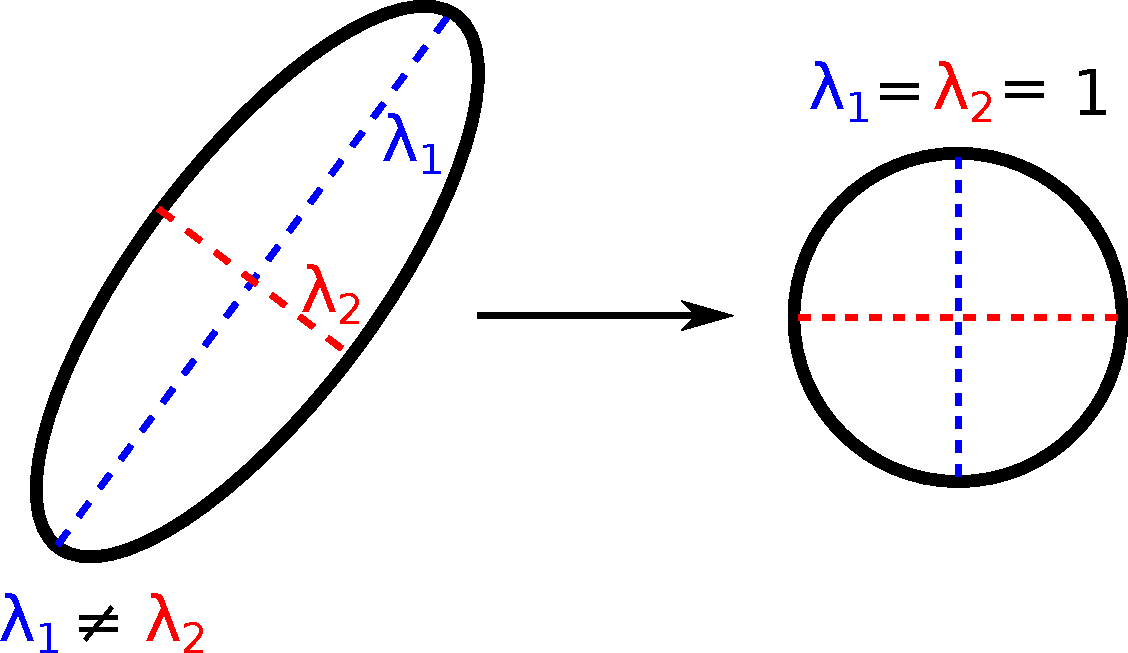
\includegraphics[width=0.5\textwidth]{figs/pca_whitening.pdf}
    \caption{Simplificação esquemática, a partir de uma perspectiva geométrica (inspirada em \citep{zafeiriou2015notes}), dos objetivos do branqueamento utilizando o PCA.}
    \label{fig:bss_pca_whitening}
\end{figure}




\begin{algorithm}[H]
    \caption{Branqueamento de dados por PCA \citep{zafeiriou2015notes}.}
    \label{alg:bss_whitening}
    \begin{algorithmic}[1]

        \State Calcular o produto escalar matricial:
        \begin{equation}
            \mathbf{X}^{T}\mathbf{X} = \sum_{i=1}^{N} \left(\mathbf{x}_{i}-\boldsymbol\mu\right)^{T}\left(\mathbf{x}_{i}-\boldsymbol\mu\right)
        \end{equation}

        \State Efetuar a auto-análise:
        \begin{equation}
            \mathbf{X}^{T}\mathbf{X} = \mathbf{V} \boldsymbol\Lambda \mathbf{V}^{T}
        \end{equation}

        \State Calcular os autovetores:
        \begin{equation}
            \mathbf{U} \leftarrow \mathbf{X} \mathbf{V} \boldsymbol\Lambda^{-\frac{1}{2}}
        \end{equation}

        \State Calcular as $d$ características:
        \begin{equation}
            \mathbf{Y} \leftarrow \mathbf{U_{d}}^{T} \mathbf{X}
        \end{equation}

        \State Rearranjar a matriz de covariância de $\mathbf{Y}$:
        \begin{equation}
            \mathbf{Y} \mathbf{Y}^{T} = \mathbf{U}^{T} \mathbf{X} \mathbf{X}^{T} \mathbf{U} = \boldsymbol\Lambda\\
        \end{equation}

        \State Obter a matriz de projeção normalizadora:
        \begin{equation}
            \mathbf{W} \leftarrow \mathbf{U} \boldsymbol\Lambda^{-\frac{1}{2}}.
        \end{equation}

    \end{algorithmic}

\end{algorithm}

Vale ressaltar o fato de que o procedimento adotado pelo Algoritmo \ref{alg:bss_whitening} carece de um único passo intermediário, que é o de manter os $n$ primeiros componentes de $\mathbf{U_{d}}$, com $n\leq d$, para ser interpretado no sentido mais amplo como, basicamente, o próprio algoritmo de Análise de Componentes Principais (\textbf{PCA}, do inglês \textit{Principal Component Analysis}) \citep{doi:10.1080/14786440109462720}.

\nomenclature{PCA}{\textit{Principal Component Analysis}}

Para fins meramente ilustrativos, uma simulação foi elaborada para mostrar os efeitos do processo de branqueamento por PCA. Para esta simulação foram utilizados dados artificialmente gerados por meio de duas variáveis aleatórias. Os dados, compostos por 2000 amostras para cada uma das variáveis envolvidas, representados no gráfico da Figura \ref{fig:bss_whitening_data_uniform} foram posicionados com base nos valores das variáveis aleatórias $X_{1}$ e $X_{2}$, que podiam variar entre -1.75 e 1.75, que foram arbitrariamente escolhidos.






\begin{figure}[H]
    \centering
    \subfloat[]{\label{fig:bss_whitening_data_uniform_a}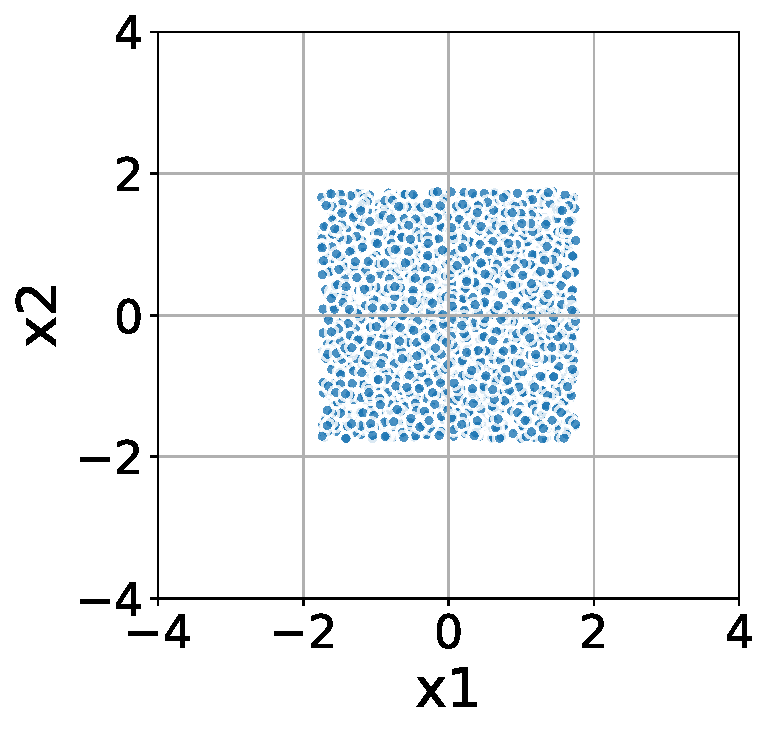
\includegraphics[width=60mm]{figs/whitening/bss_whitening_uniform.pdf}}
    \subfloat[]{\label{fig:bss_whitening_data_uniform_b}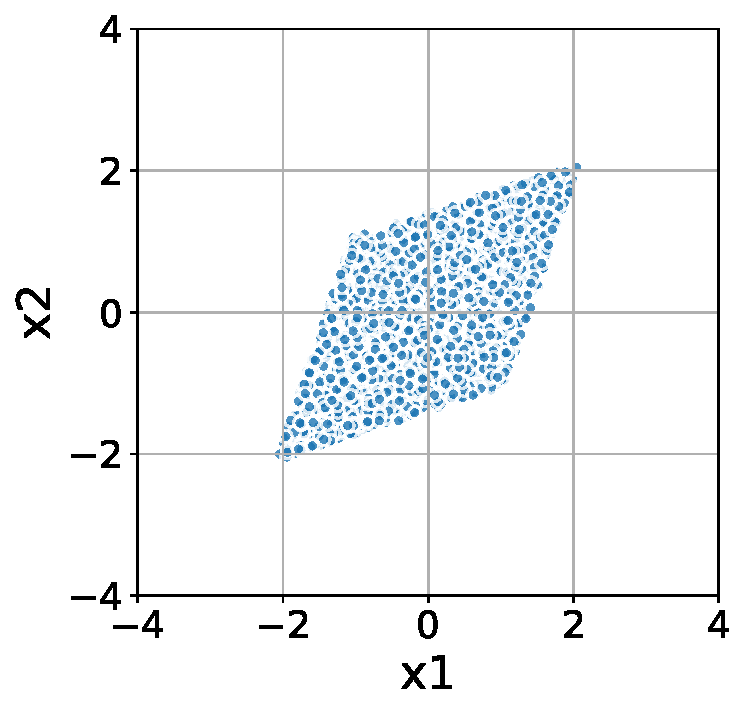
\includegraphics[width=60mm]{figs/whitening/bss_whitening_uniform_mixture.pdf}}\\
    \subfloat[]{\label{fig:bss_whitening_data_uniform_c}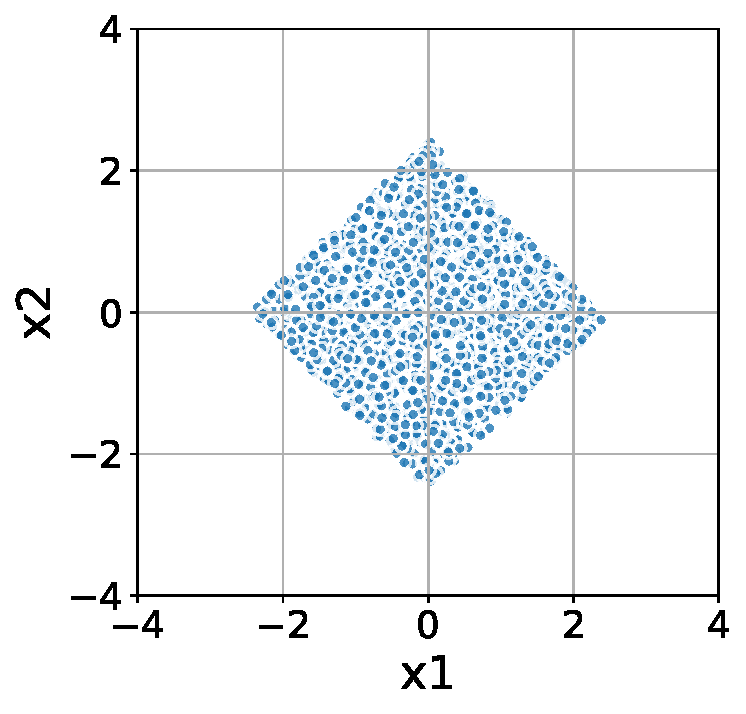
\includegraphics[width=60mm]{figs/whitening/bss_whitening_uniform_mixture_whitened.pdf}}
    \caption{(a) Distribuição uniforme de duas variáveis, (b) distribuição de misturas observadas e (c) distribuição branqueada.}
    \label{fig:bss_whitening_data_uniform}
\end{figure}



Em outra simulação, que é exibida pela Figura \ref{fig:bss_whitening_data_gaussian}, foram geradas 2000 amostras respeitando uma distribuição gaussiana de média zero e desvio padrão unitário. Observando-se as imagens da Figura \ref{fig:bss_whitening_data_gaussian} é possível compreender intuitivamente o motivo de o processo de branqueamento para o caso da distribuição gaussiana ser também conhecido como esferização (do inglês, \textit{Sphereing}).


\begin{figure}[H]
    \centering
    \subfloat[]{\label{fig:bss_whitening_data_gaussian_a}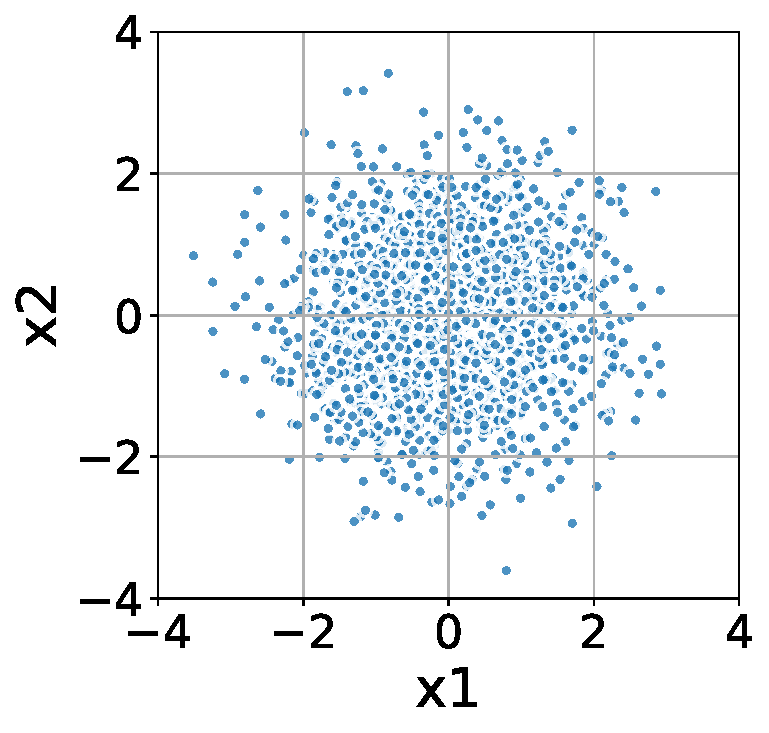
\includegraphics[width=60mm]{figs/whitening/bss_whitening_gaussian.pdf}}
    \subfloat[]{\label{fig:bss_whitening_data_gaussian_b}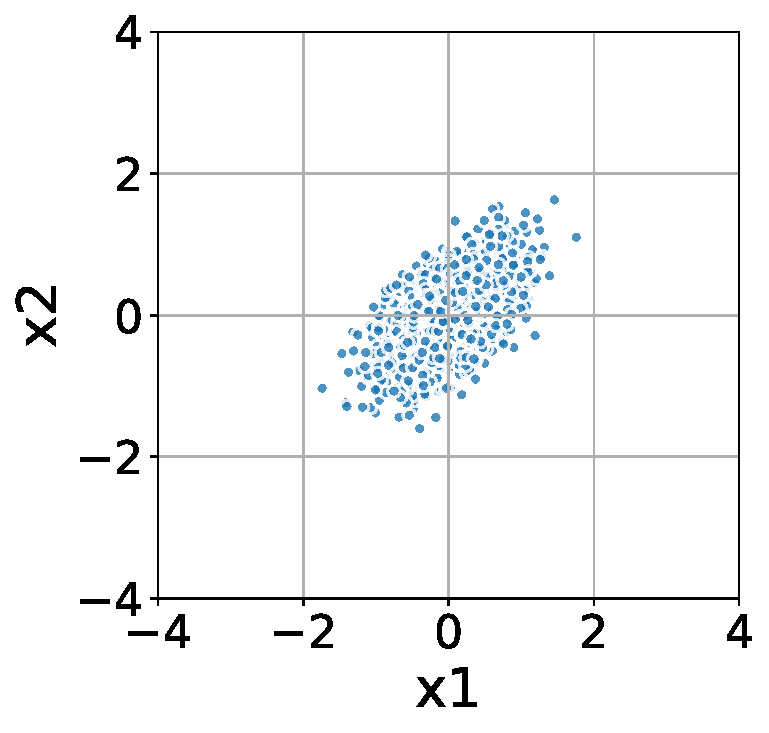
\includegraphics[width=60mm]{figs/whitening/bss_whitening_gaussian_mixture.pdf}}\\
    \subfloat[]{\label{fig:bss_whitening_data_gaussian_c}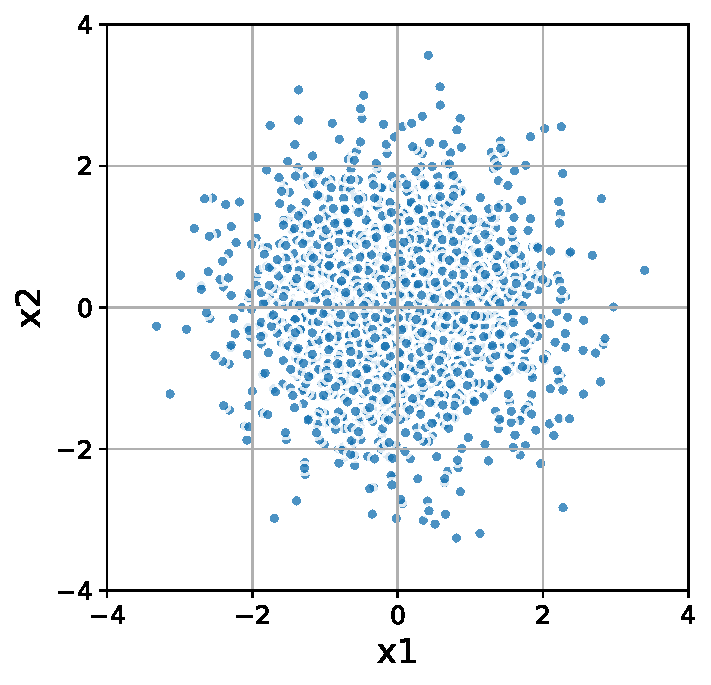
\includegraphics[width=60mm]{figs/whitening/bss_whitening_gaussian_mixture_whitened.pdf}}
    \caption{(a) Distribuição uniforme de duas variáveis, (b) distribuição de misturas observadas e (c) distribuição branqueada.}
    \label{fig:bss_whitening_data_gaussian}
\end{figure}



Uma forma de se obter os valores de $w_{ij}$ é a partir da independência estatística das misturas. A constatação de distinções que preservem uma elevada não-gaussianidade nas distribuições envolvidas pode ser explorada para efetuar eficazmente a separação dos sinais misturados com base nessa independência; a partir disso foi elaborado o método que ficou conhecido como Análise de Componentes Independentes.





Um dos princípios de estimação do ICA está associado à descorrelação não linear, obtendo-se uma matriz $\mathbf{W}$ capaz de reverter o processo de mistura, mas garantindo que todos os elementos que compõem a matriz de saída sejam, dois a dois, descorrelacionados entre si para todas as possíveis combinações, além de as transformações não lineares (cuidadosamente selecionadas), $g(y_{i})$ e $h(y_{j})$, também serem descorrelacionadas entre si.

Uma escolha apropriada das funções $g$ e $h$ é crucial para que se atinja tal objetivo, caso contrário, pode ser impraticável encontrar os componentes independentes. Assim sendo, a escolha não pode ser meramente arbitrária, aleatória ou mesmo influenciada por métodos nocivos. Existem, porém, dois métodos clássicos muito bem consolidados que ajudam a encontrar tais funções: a Estimação de Máxima Verossimilhança (\textbf{MLE}, do inglês \textit{Maximum Likelihood Estimation}) \citep{ra1922mathematical, aldrich1997ra}, oriunda da teoria de estimação; e a Informação Mútua (\textbf{MI}, do inglês \textit{Mutual Information}) \citep{cover2012elements}, advinda da teoria da informação.

\nomenclature{MLE}{\textit{Maximum Likelihood}}
\nomenclature{MI}{\textit{Mutual Information}}

Outro princípio da estimação do ICA trata-se da obtenção da máxima não-gaussianidade\footnote{Pode-se compreender não-gaussianidade como independência estatística.} possível, que pode ser estimada a partir da forma normalizada do quarto momento central da distribuição, a Curtose (do inglês \textit{Kurtosis}). A curtose mede a forma de uma dada distribuição quanto à sua ``cauda'', sendo que seu valor será igual a zero exclusivamente quando se tratar de uma legítima distribuição Gaussiana. Os casos com decaimentos laterais monotônicos suaves e com pouca (ou nenhuma) região central de planalto aproximam-se mais da distribuição Laplaciana, decaindo-se suavemente ao longo do eixo das ordenadas enquanto se caminha longamente pelo eixo das abscissas; tal caso é conhecido como Platicúrtico (ou Super-Gaussiana). Por outro lado, casos que exibam abrupto decaimento de cauda nas laterais, geralmente acompanhados de uma região central similar a um planalto, tendem a se aproximar mais da distribuição uniforme; esse caso é conhecido como Leptocúrtico (ou Sub-Gaussiana).\\

\begin{definition}[Curtose]
    Sejam o n-ésimo momento central de um sinal pode ser calculado por

    \begin{equation}
        \mu_{n} = E\left[\left(X - E\left[X\right]\right)^{n}\right]
        \vspace{0.2cm}
    \end{equation}

    \noindent e a normalização padrão dada pela divisão do momento calculado pelo desvio padrão da mesma ordem $n$ do momento em questão, ou seja,

    \begin{equation}
        \sigma^{n} = \left(\sqrt{E\left[\left(X - E\left[X\right]\right)^{2}\right]}\right)^{n}
        \hspace{0.1cm}.
        \vspace{0.2cm}
    \end{equation}

    O quarto momento central normalizado, também conhecido como Curtose, é definido por

    \begin{equation}
        k\left(X\right) = \dfrac{\mu_{4}}{\sigma^{4}} = \dfrac{E\left[\left(X - E\left[X\right]\right)^{4}\right]}{\left(E\left[\left(X - E\left[X\right]\right)^{2}\right]\right)^{2}}
        \vspace{0.2cm}
    \label{eq:bss_curtose}
    \end{equation}

\end{definition}


Mas a curtose não é a única maneira de se mensurar a não-gaussianidade; na verdade, nem mesmo é a melhor, dado que trata-se de uma métrica com elevada susceptibilidade a sofrer interferências indesejadas provocadas por \textit{Outliers}\footnote{Dados que sejam considerados aberrantes ou atípicos, sendo, portanto, passíveis de serem considerados ``fora da curva'' para eventuais considerações em modelos. Modelos mais robustos tendem a identificar tais dados e efetuar um tratamento devido para evitar que danifiquem seu desempenho.}, sobretudo por conta de seu termo de quarto grau, que faz com que até mesmo valores tipicamente considerados de magnitude não tão elevada sejam responsáveis por resultados indesejados. Isso não invalida a curtose como um recurso possível, mas o insere em um conjunto de recursos preferencialmente a serem evitados, pois suas características caminham em direção a uma instabilidade contornável.

Um dos conceitos mais importantes advindos da área de Teoria da Informação chama-se Entropia (do inglês \textit{Entropy}) de Shannon, também conhecida como \textit{informação média}, uma forma de se calcular a desordem em um contexto de teoria da informação.\\

\begin{definition}[Entropia]
    Seja $X$ uma variável aleatória. Então, a entropia de $X$, também entendida como a informação média de $X$, é dada por

    \begin{equation}
        H\left(X\right) = - \sum_{i=1}^{n}P\left(X=x_{i}\right) \log_{b} \left(P\left(X=x_{i}\right)\right)
        \hspace{0.1cm},
        \vspace{0.2cm}
        \label{eq:bss_entropy}
    \end{equation}

    \noindent sendo $P(X=x_{i})$ a probabilidade de a variável aleatória $X$ assumir o valor $x_{i}$; e, para os fins deste trabalho, $b=2$.

\end{definition}

A partir da entropia, pode-se chegar ao conceito de Negentropia\footnote{Também conhecida como \textit{sintropia} ou \textit{entropia negativa}.} (do inglês \textit{Negentropy}) \citep{schrodinger1944life, brillouin1953negentropy, mahulikar2009exact}, que trata-se de uma alternativa à curtose, contudo, consideravelmente mais robusta.\\

\begin{definition}[Negentropia]

    A negentropia de uma variável aleatória $X$ pode ser definida como

    \begin{equation}
        J\left(X\right) = H\left(X_{\text{\ gauss}}\right) - H\left(X\right)
        \hspace{0.1cm},
        \vspace{0.2cm}
        \label{eq:bss_negentropy}
    \end{equation}

    \noindent sendo que $X_{\text{\ gauss}}$ trata-se de uma variável aleatória de distribuição gaussiana e cujas média e variância são as mesmas de $X$.

\end{definition}

Tal como havia sido explicitado nesta mesma seção, a entropia pode ser utilizada como uma métrica da desordem de uma certa informação, o que permite dizer que o valor máximo de entropia caracteriza desordem máxima, ou seja, maior incerteza e, portanto, maior dificuldade de se obter uma dada informação; isso ocorre apenas no único e exclusivo caso em que a distribuição em questão se trata de uma Gaussiana. Por outro lado, entropia mínima implica maior certeza e maior facilidade para se obter a informação em questão. Efetuando-se uma análise, ainda que superficial, a respeito da Equação (\ref{eq:bss_entropy}), é possível concluir que a entropia de Shannon jamais pode ser negativa. Assim, pode-se perceber que a negentropia também sempre será não negativa. Tais características mencionadas permitem compreender a negentropia como uma espécie de distância dada pela diferença entre as distribuições envolvidas, sendo ao menos uma delas sempre uma distribuição Gaussiana \citep{suyama2007proposta}.







%   ----- ALGORITMOS NOTÁVEIS -----
\section{Algoritmos Notáveis}
\label{sec:bss_algorithms}

Conforme a área de separação de fontes avançava, foram desenvolvidos algoritmos notáveis, que são assim qualificados por conta de suas capacidades, tendo sido estudados e aprimorados em um significativo número de trabalhos publicados com contribuições de grande relevância. O princípio de otimização conhecido como \textit{maximização da informação} (\textbf{Infomax}, \textit{Information Maximization}) \citep{linsker1988self} consiste em atingir um cenário em que a entrada e a saída de uma dada função possuam a maior informação mútua possível, e trata-se da base de várias técnicas e métodos de separação de fontes.

\begin{definition}[Informação Mútua]
    Sejam X e Y duas variáveis aleatórias que componham o par (X, Y) cujos valores se encontram no espaço $\mathcal{X} \times \mathcal{Y}$, a \textit{informação mútua} entre elas será dada por 

    \begin{equation}
        I\left(X; Y\right) = \sum_{y\hspace{0.05cm} \in\hspace{0.05cm} \mathcal{Y}} \hspace{0.05cm} \sum_{x\hspace{0.05cm} \in\hspace{0.05cm} \mathcal{X}} p\left(x, y\right) \hspace{0.10cm} \log\left(\dfrac{p\left(x, y\right)}{p\left(x\right) p\left(y\right)}\right)
        \hspace{0.1cm},
        \vspace{0.2cm}
        \label{eq:bss_mutual_information}
    \end{equation}

    \noindent onde $p\left(x, y\right)$ representa a função de densidade de probabilidade conjunta de $X$ e $Y$; $p\left(x\right)$ e $p\left(y\right)$, por sua vez, representam, respectivamente, as funções de massa de probabilidade marginal de $X$ e $Y$.

\end{definition}

Alguns, como o caso do \textit{algoritmo de ponto flutuante rápido} (\textbf{FastICA}, \textit{Fast Fixed-Point Algorithm}) \citep{761722} --- que, em busca da maximização de alguma métrica de não-gaussianidade\footnote{Lembrando que a não-gaussianidade pode ser interpretada como uma forma de independência estatística.}, rotaciona ortogonalmente dados pré-branqueados --- tornaram-se mais famosos, sobretudo por conta de seu considerável ganho de eficiência sobre uma técnica já bastante utilizada pela comunidade de separação de fontes. Outro método importante para o avanço desta técnica é o \textbf{RobustICA} \citep{5356190}, uma sutil variação do FastICA, otimizando o contraste da curtose, mas que exibe maiores robustez e velocidade de convergência.

Uma abordagem um pouco diferente, chamada de \textit{identificação cega de quarta ordem} (\textbf{FOBI}, \textit{Fourth Order Blind Identification}) \citep{cardoso1989source, miettinen2015fourth}, utiliza-se de momentos (estatísticos) de quarta ordem para realizar o processo de separação de sinais. Outra abordagem, computacionalmente mais parcimoniosa, é a do algoritmo conhecido como \textit{identificação cega de segunda ordem} (\textbf{SOBI}, \textit{Second Order Blind Identification}) \citep{554307}, que explora momentos de segunda ordem e depende de as fontes serem individualmente correlacionadas no tempo, mas mutuamente descorrelacionadas. Para a realização do SOBI, é preciso realizar etapas de branqueamento dos dados, computação de matrizes de correlação atrasada, e diagonalização conjunta. 

O método \textit{diagonalização conjunta aproximada de auto-matrizes} (\textbf{JADE}, \textit{Joint Approximation Diagonalization of Eigen-matrices}) \citep{cardoso1999high} explora momentos de quarta ordem e também está entre os mais amplamente explorados em trabalhos da área de separação de fontes. É importante lembrar que não há um único método que seja o melhor para todo os possíveis cenários, portanto, é sempre válido averiguar qual método se encaixa melhor para o cenário a ser trabalhado; há, contudo, alguns bons trabalhos que fazem tais investigações, confrontando alguns dos mais conhecidos métodos para esta finalidade \citep{matic2009comparison, sahonerocomparison}.










%   ---------------
%   ----- SCA -----
%   ---------------
\section{Análise de Componentes Esparsos}
\label{sec:bss_sca}

Além da técnica ICA, existem outras técnicas que também efetuam uma análise de componentes e que podem ser exploradas com o intuito de se realizar a tarefa de separação de sinais; esta seção abordará mais especificamente a Análise de Componentes Esparsos (\textbf{SCA}, do inglês \textit{Sparse Component Analysis}). Contudo, antes mesmo de prosseguir para questões mais aprofundadas sobre tal técnica, pode ser importante começar explicando-se o significado de esparso. A ideia de esparsidade está intimamente relacionada à ideia de dispersão e distanciamento, podendo ser interpretada, portanto, como o oposto de densidade. A esparsidade pode, inclusive, ser quantificada, segundo o que se entende por grau de esparsidade de uma matriz.\\

\nomenclature{SCA}{\textit{Sparse Component Analysis}}

\begin{definition}[Grau de Esparsidade]
    Seja uma matriz $\bm{M}$ definida por

    \begin{equation}
        M =
        \left[\begin{array}{cccc}
        m_{11} & m_{12} & \cdots & m_{1n} \\
        m_{21} & m_{22} & \cdots & m_{2n} \\
        \vdots & \vdots & \ddots & \vdots \\
        m_{n1} & m_{n2} & \cdots & m_{nn}
        \end{array}\right].
    \end{equation}

    Considerando-se $N$ como o número de elementos nulos da matriz e $T$ como o número total de elementos da matriz, o Grau de Esparsidade, $E$, pode ser obtido a partir de

    \begin{equation}
        E = \dfrac{N}{T}
        \hspace{0.2cm}\cdot
        \label{eq:bss_sparsity}
    \end{equation}

    \label{def:sparsity}
\end{definition}

Pela definição, em um cenário ideal, a matriz $M$ seria composta por valores não nulos exclusivamente em sua diagonal principal, ou seja, em $m_{11}, m_{22}, \dots , m_{nn}$; e, dado que uma das vantagens de se trabalhar com matrizes esparsas advém do fato de ser possível armazenar apenas os valores não nulos das matrizes, isso significa que, para este caso em particular, apenas os valores da diagonal principal seriam armazenados. Para que seja possível trabalhar com matrizes em tal situação, são necessárias técnicas especiais de armazenamento e processamento, por exemplo, pelo uso de listas de coordenadas; tais técnicas computacionais, no entanto, não serão minuciosamente exploradas ou explanadas neste trabalho.

Em situações um pouco mais próximas ao que se encontra na realidade, as matrizes não são tão esparsas assim. Além de haver diversos elementos não nulos em posições que não sejam a diagonal principal, é possível que os próprios valores que devam ser considerados como nulos não sejam originalmente iguais a zero, o que dependeria de alguma técnica de pré-processamento que ajustasse tais valores com base em algum Limiar (do inglês \textit{Threshold}), podendo resultar em um aumento considerável da esparsidade da matriz. As técnicas de análise de componentes esparsos possuem características geométricas intrínsecas que as favorecem em casos de cenários subparametrizados \citep{theis2003linear}, ou seja, cenários em que o número de misturas observadas é inferior ao número de fontes.

O Algoritmo \ref{alg:bss_sca} é uma versão bastante simplificada que explica sucintamente os quatro passos básicos essenciais de uma técnica de SCA. A versão simplificada pode ser útil para oferecer uma visão superficial do caminho a ser trilhado. Contudo, a explicação acerca de tal algoritmo ainda será um pouco mais aprofundada ainda nesta mesma seção; não haverá um detalhamento matemático muito rigoroso, mas serão fornecidas fontes de referência que poderão ser consultadas para o caso de os objetivos do leitor dependerem de tal abordagem. \\

\begin{algorithm}[H]
    \caption{Versão simplificada da Análise de Componentes Esparsos (SCA) \citep{gribonval2006survey}.}
    \label{alg:bss_sca}
    \begin{algorithmic}[1]

        \State Aplicar transformação linear esparsificante à mistura.

        \State Estimar $\bm{A}$ a partir da dispersão de $C_{\bm{x}}$.

        \State Estimar as representações da fonte.

        \State Reconstruir as fontes a partir da inversa de uma transformação esparsificante.

    \end{algorithmic}

\end{algorithm}

Dando continuidade às explicações um pouco mais minuciosas sobre o SCA, tomando como base ainda o Algoritmo \ref{alg:bss_sca}, pode ser interessante começar pelo fato de que a análise será feita individualmente, uma a uma, para cada mistura observada; ou seja, caso haja três sinais observados resultantes de misturas, serão necessárias três execuções completas do algoritmo para que seja possível realizar a tarefa almejada de separação de sinais. Observe que a primeira etapa do algoritmo se refere à aplicação de uma transformação linear esparsificante à mistura observada, que é a entrada do algoritmo. É muito comum que a escolha dessa transformação esparsificante seja feita entre Transformada Discreta Wavelet (\textbf{DWT}, do inglês \textit{Discrete Wavelet Transform}) e a Transformada de Fourier de Tempo Curto (\textbf{STFT}, do inglês \textit{Short-Time Fourier Transform}).

\nomenclature{DWT}{\textit{Discrete Wavelet Transform}}
\nomenclature{STFT}{\textit{Short-Time Foutier Transform}}






%   ---------------
%   ----- NMF -----
%   ---------------
\section{Fatoração de Matrizes Não-Negativas}
\label{sec:bss_nmf}

Assim como ocorre com outros casos mencionados neste trabalho, a Fatoração de Matrizes Não Negativas (\textbf{NMF}, do inglês \textit{Non-Negative Matrix Factorization}), introduzida em \citep{1781640}, não se trata de um algoritmo em si; em vez disso, trata-se de uma técnica que pode ser compreendida de maneira quase autoexplicativa a partir de seu nome, ou seja, independentemente de qual seja o algoritmo para se atingir tal objetivo, a ideia é a de se obter duas matrizes de valores não negativos que, multiplicando-se uma pela outra, obtém-se a matriz resultante que se deseja representar ao fim.

\nomenclature{NMF}{\textit{Non-Negative Matrix Factorization}}

O objetivo de se efetuar tal processo de decomposição matricial é, principalmente, o de facilitar a análise dos resultados obtidos, mas cabe aqui ressaltar o fato de que nem todos os casos são plenamente solucionáveis. Pode ser preciso trabalhar com aproximações, mas isto não significa que os resultados sejam necessariamente imprecisos e inacurados.

Os artigos \citep{lee1999learning} e \citep{Lee:2000:ANM:3008751.3008829} foram alguns dos principais responsáveis pelas amplas divulgação, adesão e desenvolvimento dos algoritmos de NMF pelo mundo. Esse desenvolvimento passou a ser bastante conveniente para aplicações de áudio por motivos como o fato de o ICA ser mais eficaz para aplicações envolvendo um número de sensores tão grande quanto o número de fontes, o que nem sempre é possível; o NMF, por outro lado, não sofre com tal dependência de forma tão intensa, o que permite que esta abordagem seja explorada com maiores chances de sucesso para casos com limitação de canais, muito comuns quando se trabalha com música, dado que tipicamente são encontrados casos com \textit{Mono} (1 canal) ou \textit{Stereo} (2 canais).
